\section{Расчетная сетка}

Сложность численного расчета данной задачи следующая. При применении метода конечных элементов к данной задаче возникают затруднения, связанные с тем,
что искомый потенциал поля имеет особенность (уходит на бесконечность) в окрестности источника тока.
Это приводит к необходимости сгущения расчётной сетки в этой окрестности, но сильное сгущение
приводит к чрезмерному росту числа узлов сетки и, как следствие, сильному росту времени, требуемому на решение.

Поэтому представляет актуальность задача построения оптимальной сетки, в которой сочетаются высокая точность
получаемого решения и малое число узлов.

\subsection{Постановка задачи}

В качестве модельной рассматривалась задача для трёхслойной осесимметричной модели системы скважина--пласт:
задача рассматривается в цилиндрической системе координат ${(r, z)}$, где ${r > 0}$ --- радиальная координата,
${z}$ --- осевая координата, по которой область однородна (единственный однородный пласт бесконечной мощности),
первый слой --- сама скважина (${0 < r < 1}$) с УЭС ${\rho_\text с = 1}$, второй слой --- зона проникновения (${1<r<r_\text{зп} = 9}$)
с УЭС ${\rho_\text{зп}=15}$, третий слой --- пласт (${r>r_\text{п}}$) с УЭС ${\rho_\text{п}=10}$. В начале координат размещается
источник тока силой 1.

В качестве основы для расчётной сетки использовалась одномерная сетка, узлы которой рассчитаны в параграфе
\ref{OneDim}, отложенная на лучах, исходящих из начала координат под различными углами.
Затем эта основа дополнялась узлами, лежащими на границах разрыва УЭС ${r=1}$ и ${r=r_\text{п}}$.
Также производилось дополнительное адаптивное сгущение сетки в областях, в которых наблюдалось сильное искажение
решения по сравнению с эталонным (полученным на сетке с большим числом узлов во всей области).

\subsection{Построение одномерной сетки}
\label{OneDim}

Задача БКЗ моделируется, как правило, для осесимметричного случая, что приводит к двумерным задачам.
Известно, что точное решение (потенциал электрического поля) для случая одинакового во всём пространстве
УЭС есть константа, делённая на расстояние до источника:

$$\varphi(r, z)=\frac{C}{\sqrt{r^2+z^2}}$$ (здесь начало координат совпадает с источником тока)

Поскольку для любого распределения УЭС решение в малой окрестности источника тока практически определяется
УЭС в этой же окрестности (а она считается постоянной, равной УЭС жидкости в скважине), решение будет всегда
иметь одну и ту же особенность в начале координат и изменяться плавно вдали от источника тока.
В качестве первого приближения к оптимальной сетке можно использовать оптимальную одномерную сетку
для известного распределения ${y=1/x}$, и затем эту одномерную сетку распространять на несколько лучей,
исходящих из начала координат.

Поэтому первой поставленной задачей было построение оптимальной одномерной сетки для интерполяции
известной функции ${y=1/x}$:

{\bf Задача}. Дана функция ${y=1/x}$ на интервале ${[\delta, +\infty)}$ (${\delta > 0}$). Построить на ней сетку
${\{x_i,\,i=0,1,\dots\}}$ из наименьшего числа узлов (начиная с ${x_0=\delta}$) так, чтобы разность между
функцией ${y}$ и приближающим её сплайном первого порядка на этой сетке не превышала заданного значения
${\varepsilon}$.

%Тут краткий обзор, что использовалось для решения, формулы, программы.
%URL-ссылка офомляется так: \cite{Python}
\def\ibreak{& \\ &}
\def\iline{& \\ \cline{1-2} &}

\makeatletter
\newenvironment{customenv}
  {\align &} % \start@align\@ne\st@rredtrue\m@ne
  {& \endalign}

\newenvironment{systemed}
  {\left\{ \begin{aligned} &}
  {& \end{aligned} \right.}

\newenvironment{totalited}
  {\left[ \begin{aligned} &}
  {& \end{aligned} \right.}


Математическая постановка:
\begin{customenv}
  f(x) = \frac 1 x \text{ --- исходная функция}
  \nonumber
  \ibreak
  X = ( x_i ) \, , \, i \in [0,N] \text{ --- сетка}
  \nonumber
  \ibreak
  x_0 = \delta \text{ --- известное}
  \nonumber
\end{customenv}
\begin{customenv}
  F(x) = \begin{totalited}
    F_0(x) \, , && x \in [x_0, x_1]
    \ibreak
    F_1(x) \, , && x \in [x_1, x_2]
    \ibreak
    \dots &&
    \ibreak
    F_{N-1}(x) \, , && x \in [x_{N-1}, x_N]
  \end{totalited}
  \ibreak
  F_i(x) = A_i \, x + B_i \, , \, x \in [x_i, x_{i+1}]
\end{customenv}
\begin{equation}
  \begin{systemed}
    F_i(x_i) = f(x_i)
    \ibreak
    F_i(x_{i+1}) = f(x_{i+1})
  \end{systemed}
  \Rightarrow
  A_i, B_i
\end{equation}
\begin{customenv}
  R(x) = \begin{totalited}
    R_0(x) \, , && x \in [x_0, x_1]
    \ibreak
    R_1(x) \, , && x \in [x_1, x_2]
    \ibreak
    \dots &&
    \ibreak
    R_{N-1}(x) \, , && x \in [x_{N-1}, x_N]
  \end{totalited}
  \ibreak
  R_i(x) = \left| F_i(x) - f(x) \right|, \, x \in [x_i, x_{i+1}]
\end{customenv}
\begin{customenv}
  R'_i(x) = 0 \, \Rightarrow \, x_\text{max}
  \ibreak
  R_i(x_\text{max}) = \varepsilon \, \Rightarrow \, x_{i+1}
\end{customenv}

Решение:
\begin{customenv}
  \begin{systemed}
    F_i(x_i) = f(x_i)
    \ibreak
    F_i(x_{i+1}) = f(x_{i+1})
  \end{systemed}
  \Rightarrow
  \begin{systemed}
    A_i \, x_i + B_i = f(x_i)
    \ibreak
    A_i \, x_{i+1} + B_i = f(x_{i+1})
  \end{systemed}
  \Rightarrow
  \nonumber
  \ibreak
  \begin{systemed}
    A_i = \frac {f(x_{i+1}) - f(x_i)} {x_{i+1} - x_i}
    \ibreak
    B_i = f(x_i) - A_i \, x_i
  \end{systemed}
\end{customenv}
\begin{customenv}
  R_i(x) = A_i \, x + B_i - \frac 1 x 
  \ibreak
  R'_i(x) = A_i + \frac 1 {x^2} = 0
  \, \Rightarrow \,
  x_\text{max} = \frac 1 {\sqrt{-A_i}}
  \ibreak
  R_i(x_\text{max}) =
  A_i \, \frac 1 {\sqrt{-A_i}} + B_i - \sqrt{-A_i} = \varepsilon
  \, \Rightarrow
  \label{eq:sympy}
\end{customenv}
\begin{equation}
  x_{i+1} = \begin{totalited}
    \frac{\varepsilon x_{i}^{2} + x_{i} - 2 \sqrt{\varepsilon x_{i}^{3}}}{\varepsilon^{2} x_{i}^{2} - 2 \varepsilon x_{i} + 1},
    && \text{ --- выражение для нового левого узла}
    \ibreak
    \frac{\varepsilon x_{i}^{2} + x_{i} + 2 \sqrt{\varepsilon x_{i}^{3}}}{\varepsilon^{2} x_{i}^{2} - 2 \varepsilon x_{i} + 1};
    && \text{ --- выражение для нового правого узла}
  \end{totalited}
\end{equation}

Решение уравнения \eqref{eq:sympy} было получено посредством библиотеки Sympy в Python.


\newcommand{\addtwoimg}[3]{

  \begin{figure}[H]

  \begin{subfigure}{0.5\textwidth}
  \includegraphics[page=1]{#1} 
  \caption{Источник потенциала}
  \end{subfigure}
  \begin{subfigure}{0.5\textwidth}
  \includegraphics[page=2]{#1}
  \caption{Система}
  \end{subfigure}

  \caption{#2}
  \label{#3}

  \end{figure}

}

\renewcommand{\addimg}[3]{
  \begin{figure}[H]
    \includegraphics{#1}
    \caption{#2} \label{#3}
  \end{figure}
}

\newcommand{\addimgexp}[1]{
  % \makeatletter
  %   \def\meshfn{exps/}
  %   \g@addto@macro\meshfn{#1}
  %   \g@addto@macro\meshfn{_mesh}

  %   \def\solvefn{exps/}
  %   \g@addto@macro\solvefn{#1}
  %   \g@addto@macro\solvefn{_solve}

  %   \def\rhogfn{exps/}
  %   \g@addto@macro\rhogfn{#1}
  %   \g@addto@macro\rhogfn{_rhog}
  % \makeatother

  % \makeatletter
  %   \g@addto@macro\meshlabel{#1}
  %   \g@addto@macro\meshlabel{_mesh}

  %   \g@addto@macro\solvelabel{#1}
  %   \g@addto@macro\solvelabel{_solve}

  %   \g@addto@macro\rhoglabel{#1}
  %   \g@addto@macro\rhoglabel{_rhog}
  % \makeatother

  \addtwoimg{exps/#1_mesh}{Триангуляция}{fig:#1_mesh}
  \addtwoimg{exps/#1_solve}{Решение потенциального поля}{fig:#1_solve}
  \addimg{exps/#1_rhog}{Кажущееся сопротивление}{fig:#1_rhog}
}


\subsection{Построение двумерной сетки}

%Краткое описание экспериментов, ссылки на литературу, библиотеки (triangle и др.).

Для построения вершин шестиугольников использованы одномерные сетки: узлы решения для гиперболы
и узлы, равноотстоящие в логарифмическом масштабе.
Использована реализация триангуляции библиотеки triangle на Python c различными настройками:
режимы добавления новых узлов, учет графа, значения ограничения снизу значений углов треугольников.

\newcounter{exp}

\refstepcounter{exp} \theexp \label{text_fullmesh}.
Построены вершины шестиугольников из узлов решения для гиперболы.
На рис. \ref{fig:fullmesh_1}--\ref{fig:fullmesh_2} построены отрезки графа внутреннего и внешнего границ (граф изображен с красным цветом)
и обозначена метка дыры (изображена красным крестиком), в которой исключена триангуляция.
Вызвана триангуляция библиотеки triangle с настройкой 'pq30',
где 'p' сообщает библиотеке о вводе графа, 'q30' --- ограничение снизу 30 градусов значений углов треугольников триангуляции.

421 узлов.

\addtwoimg{exps/fullmesh_1}{Триангуляция}{fig:fullmesh_1}
\addimg{exps/fullmesh_2}{Триангуляция}{fig:fullmesh_2}

\stepcounter{exp} \theexp.
Для расчетной сетки выбраны узлы, расположенные справа от оси ${r = 0}$,
и построены сегменты половинов внутреннего и внешнего границ,
Использованы лагранжевые элементы ${\mathcal{P}_1}$ (рис. \ref{fig:1_mesh}--\ref{fig:1_rhog}).

Большая погрешность, негладкость \ref{fig:1_rhog}. 221 узлов в триангуляции.

\addimgexp{1}

\stepcounter{exp} \theexp.
Использованы узлы, равноотстоящие в логарифмическом масштабе (рис. \ref{fig:2_mesh}--\ref{fig:2_rhog}).

Большая погрешность, негладкость на рис. \ref{fig:2_rhog}. 1510 узлов в триангуляции.

\addimgexp{2}

\stepcounter{exp} \theexp.
Добавлены сегменты на местах разрыва коэффициента УЭС (рис. \ref{fig:3_mesh}--\ref{fig:3_rhog}).

Погрешность большая, негладкость подобия осцилляции на рис. \ref{fig:3_rhog}. 7201 узлов в триангуляции.

\addimgexp{3}

\stepcounter{exp} \theexp.
Использованы лагранжевые элементы ${\mathcal{P}_3}$ (рис. \ref{fig:4_mesh}--\ref{fig:4_rhog}).

Погрешность меньшая, негладкость подобия осцилляции на рис. \ref{fig:4_rhog}. 7201 узлов в триангуляции.

\addimgexp{4}

\refstepcounter{exp} \theexp \label{optimal}.
Использован точечный источник вместо внутреннего граничного условия  (рис. \ref{fig:5_mesh}--\ref{fig:5_rhog}).

Погрешность меньшая, негладкость подобия осцилляции на рис. \ref{fig:5_rhog}. 6659 узлов в триангуляции.

\addimgexp{5}

\stepcounter{exp} \theexp.
Добавлены на границе ${r = 0}$ узлы одномерной сетки (рис. \ref{fig:6_mesh}--\ref{fig:6_rhog}).

Погрешность меньшая, негладкость подобия осцилляции на рис. \ref{fig:6_rhog}. 6845 узлов в триангуляции.

\addimgexp{6}

\refstepcounter{exp} \theexp.
Добавлены сегменты возле мест разрыва коэффициента УЭС. Использованы лагранжевые элементы ${\mathcal{P}_2}$
(рис. \ref{fig:7_mesh}--\ref{fig:7_rhog}).

Практически идеальный результат на рис. \ref{fig:7_rhog}. 156856 узлов в триангуляции.

\addimgexp{7}

\refstepcounter{exp} \theexp \label{best}.
Использованы узлы, равноотстоящие в логарифмическом масштабе;
узлы лежащие в местах пересечений границ областей УЭС с концентрическими окружностями и лучами,
отрезки графа на местах разрыва коэффициента УЭС; лагранжевые элементы ${\mathcal{P}_2}$; настройка 'p' библиотеки triangle
(рис. \ref{fig:8_mesh_1}--\ref{fig:8_rhog}).

Практически идеальный результат на рис. \ref{fig:8_rhog}. 2859 узлов в триангуляции.

\begin{figure}[H]
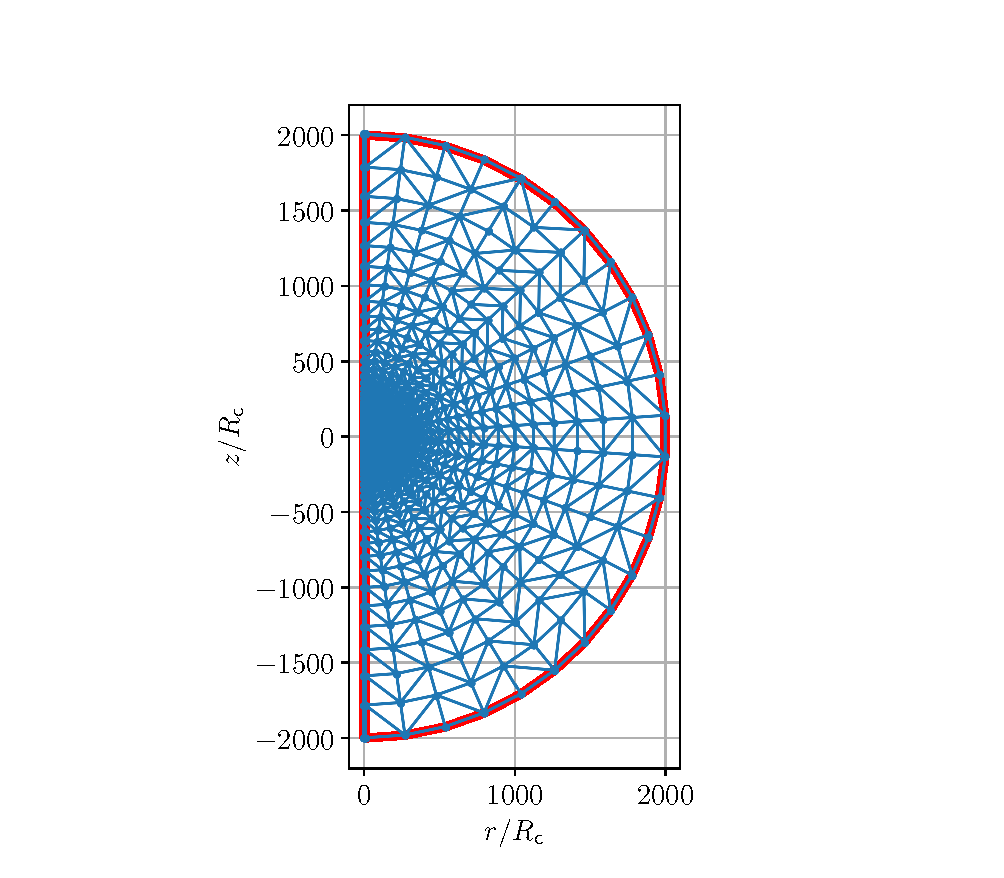
\includegraphics{exps/last_tg_1}
\caption{Триангуляция}
\label{fig:8_mesh_1}
\end{figure}

\begin{figure}[H]
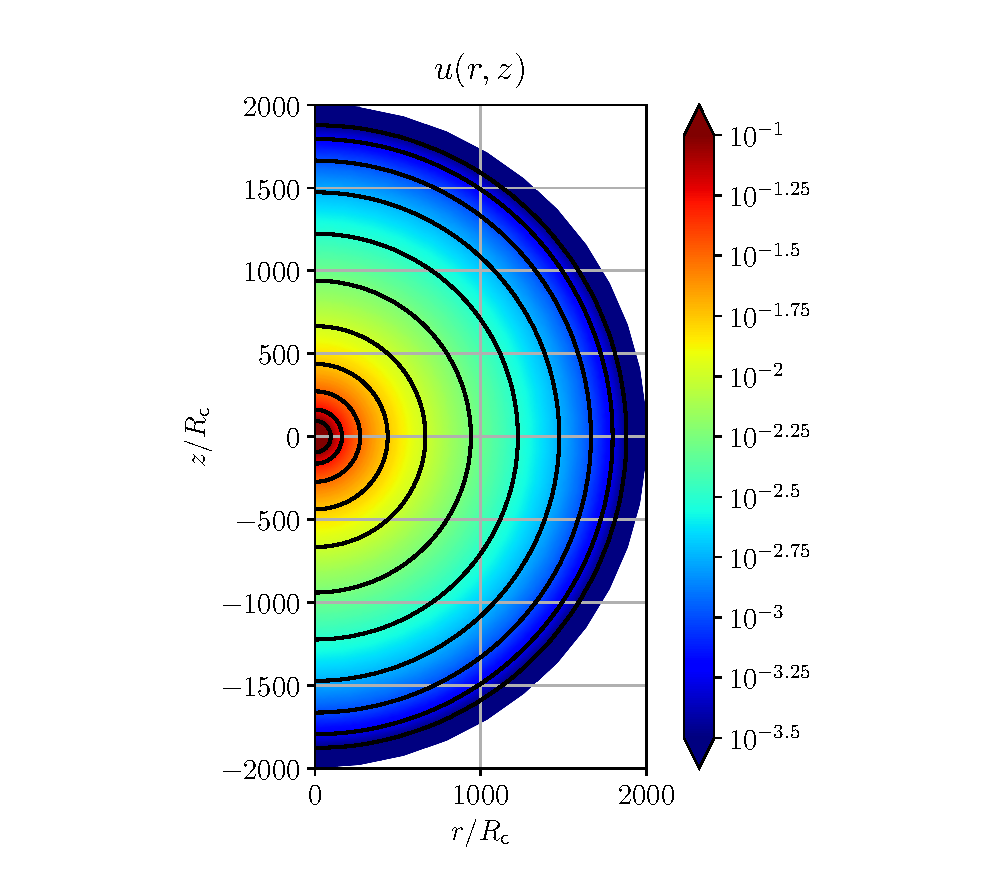
\includegraphics{exps/last_field_1}
\caption{Решение потенциального поля}
\label{fig:8_field_1}
\end{figure}

\begin{figure}[H]
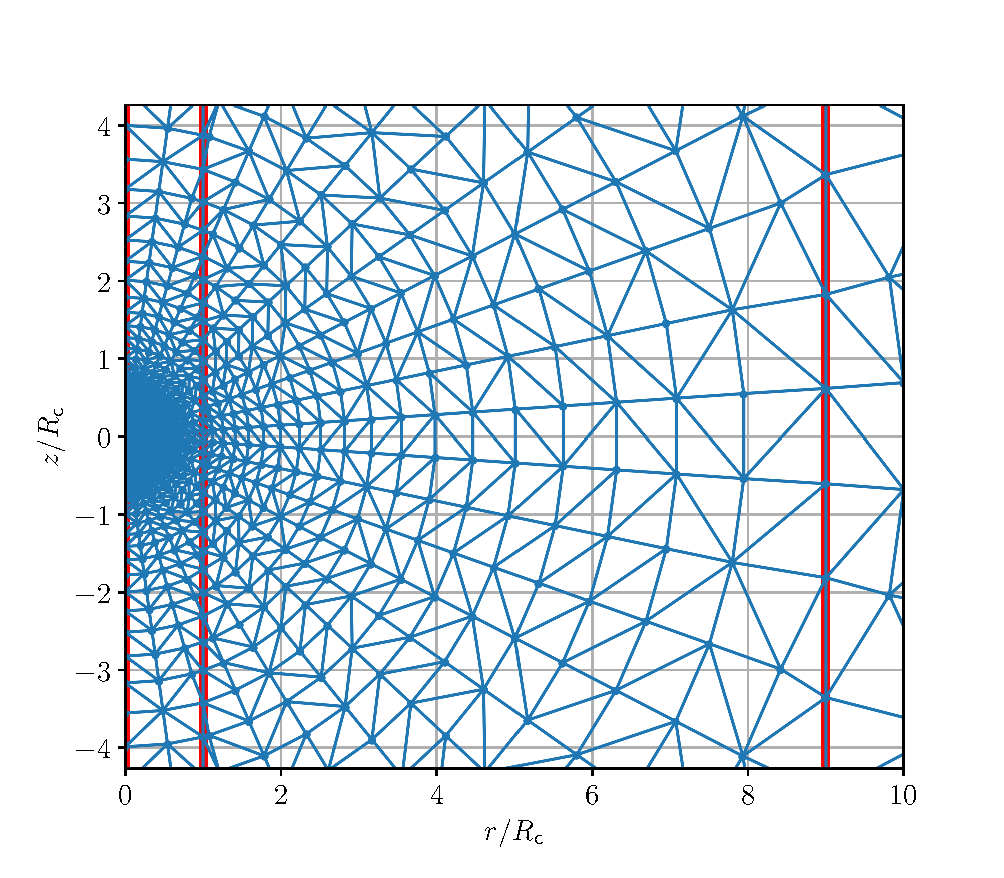
\includegraphics{exps/last_tg_2}
\caption{Триангуляция}
\label{fig:8_mesh_2}
\end{figure}

\begin{figure}[H]
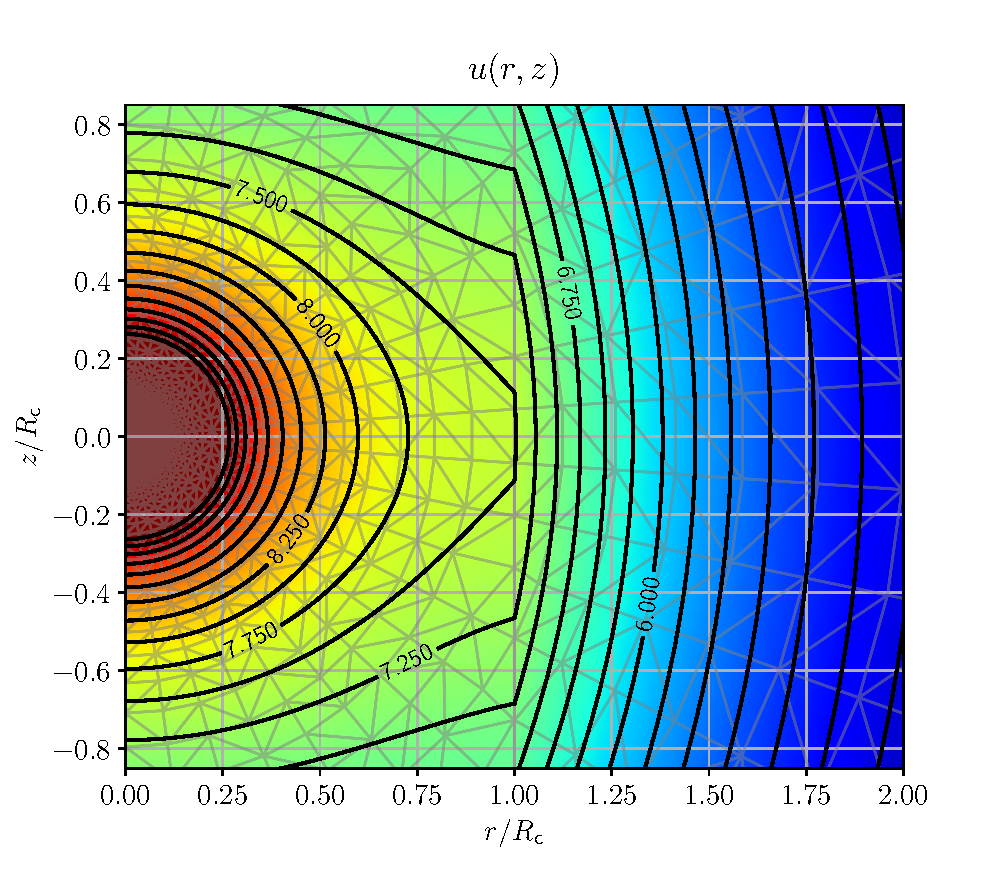
\includegraphics{exps/last_field_2}
\caption{Решение потенциального поля}
\label{fig:8_field_2}
\end{figure}

На рис. \ref{fig:8_field_2} наблюдается разрыв градиента потенциального поля на границе области скважины
и сингулярность поля в точке источника потенциала,
означает, что это не классичекое решение задачи, а более общее -- обобщенное решение задачи. 

\begin{figure}[H]
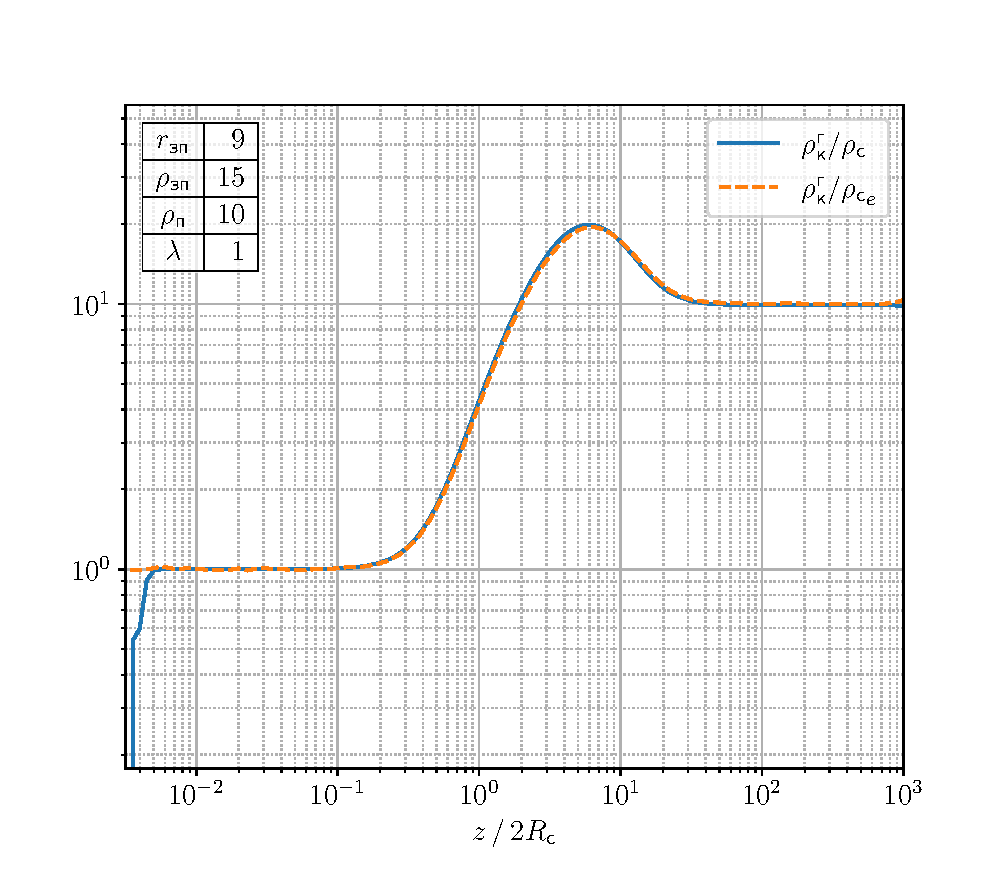
\includegraphics{exps/last_curves}
\caption{Кажущееся сопротивление}
\label{fig:8_rhog}
\end{figure}


\subsection{Результаты}

Оптимальный результат получен в эксперименте \ref{best} за ${538 \text{ мc } \pm 37.8 \text{ мс }}$, 7 проходов
(${\text{среднее значение} \pm \text{среднеквадратичное отклонение}}$ от 7 проходов, в каждом проходе 1 цикл). Использованы узлы, равноотстоящие в логарифмическом масштабе; узлы лежащие в местах пересечений границ областей УЭС с концентрическими окружностями и лучами, отрезки графа на местах разрыва коэффициента УЭС; лагранжевые элементы ${\mathcal{P}_2}$; настройка 'p' библиотеки triangle. Использован компьютер для вычисления: операционная система Ubuntu 18.04 LTS, процессор Intel Pentium 4415U 2.30 ГГц с 4 логическими процессорами ($1 \text{ физический процессор} \times 2 \text{ ядра в физическом процессоре} \times 2 \text{ потока в каждом ядре}$)..

В результате проведённых численных экспериментов разработан метод построения оптимальных сеток для решения задачи БКЗ на сетке, позволяющий получить приемлимое численное решение с меньшими затратами ресурсов. В данном случае мы следили за двумя параметрами: гладкостью решения и сравнением "на глаз" с известной палеткой. Поскольку принятая методика решения обратной задачи БКЗ основано на использованием палеток на "сравнении на глаз", то такой критерий годится. Относительная ошибка примерно ${<10}$ \%.

\clearpage